%%
%% This is file `sample-acmsmall.tex',
%% generated with the docstrip utility.
%%
%% The original source files were:
%%
%% samples.dtx  (with options: `acmsmall')
%% 
%% IMPORTANT NOTICE:
%% 
%% For the copyright see the source file.
%% 
%% Any modified versions of this file must be renamed
%% with new filenames distinct from sample-acmsmall.tex.
%% 
%% For distribution of the original source see the terms
%% for copying and modification in the file samples.dtx.
%% 
%% This generated file may be distributed as long as the
%% original source files, as listed above, are part of the
%% same distribution. (The sources need not necessarily be
%% in the same archive or directory.)
%%
%% Commands for TeXCount
%TC:macro \cite [option:text,text]
%TC:macro \citep [option:text,text]
%TC:macro \citet [option:text,text]
%TC:envir table 0 1
%TC:envir table* 0 1
%TC:envir tabular [ignore] word
%TC:envir displaymath 0 word
%TC:envir math 0 word
%TC:envir comment 0 0
%%
%%
%% The first command in your LaTeX source must be the \documentclass command.
\documentclass[sigplan]{acmart}
%% NOTE that a single column version is required for 
%% submission and peer review. This can be done by changing
%% the \doucmentclass[...]{acmart} in this template to 
%% \documentclass[manuscript,screen]{acmart}
%% 
%% To ensure 100% compatibility, please check the white list of
%% approved LaTeX packages to be used with the Master Article Template at
%% https://www.acm.org/publications/taps/whitelist-of-latex-packages 
%% before creating your document. The white list page provides 
%% information on how to submit additional LaTeX packages for 
%% review and adoption.
%% Fonts used in the template cannot be substituted; margin 
%% adjustments are not allowed.
%%
%% \BibTeX command to typeset BibTeX logo in the docs
\AtBeginDocument{%
  \providecommand\BibTeX{{%
    \normalfont B\kern-0.5em{\scshape i\kern-0.25em b}\kern-0.8em\TeX}}}

%% Rights management information.  This information is sent to you
%% when you complete the rights form.  These commands have SAMPLE
%% values in them; it is your responsibility as an author to replace
%% the commands and values with those provided to you when you
%% complete the rights form.
\setcopyright{acmcopyright}
\copyrightyear{2022}
\acmYear{2022}
\acmDOI{XXXXXXX.XXXXXXX}


%%
%% These commands are for a JOURNAL article.
\acmJournal{JACM}
\acmVolume{37}
\acmNumber{4}
\acmArticle{111}
\acmMonth{8}

%%
%% Submission ID.
%% Use this when submitting an article to a sponsored event. You'll
%% receive a unique submission ID from the organizers
%% of the event, and this ID should be used as the parameter to this command.
%%\acmSubmissionID{123-A56-BU3}

%%
%% The majority of ACM publications use numbered citations and
%% references.  The command \citestyle{authoryear} switches to the
%% "author year" style.
%%
%% If you are preparing content for an event
%% sponsored by ACM SIGGRAPH, you must use the "author year" style of
%% citations and references.
%% Uncommenting
%% the next command will enable that style.
%%\citestyle{acmauthoryear}

%%
%% Personal package imports
\usepackage{listings}
\usepackage{multirow}
\usepackage{dirtytalk} %quotations
\usepackage{courier}

% TODO: remove me
\usepackage{todonotes}
\setuptodonotes{inline}

% listing settings
\lstset{basicstyle=\footnotesize\ttfamily}

%%
%% end of the preamble, start of the body of the document source.
\begin{document}

%%
%% The "title" command has an optional parameter,
%% allowing the author to define a "short title" to be used in page headers.
\title[Void Processes]{Void Processes: Minimising privilege by default}

%%
%% The "author" command and its associated commands are used to define
%% the authors and their affiliations.
%% Of note is the shared affiliation of the first two authors, and the
%% "authornote" and "authornotemark" commands
%% used to denote shared contribution to the research.
\author{Jake Hillion}
\affiliation{%
  \institution{University of Cambridge}
  \country{United Kingdom}
}
\email{jake.hillion@cl.cam.ac.uk}

%%
%% By default, the full list of authors will be used in the page
%% headers. Often, this list is too long, and will overlap
%% other information printed in the page headers. This command allows
%% the author to define a more concise list
%% of authors' names for this purpose.
%\renewcommand{\shortauthors}{Hillion}

%%
%% The abstract is a short summary of the work to be presented in the
%% article.
\begin{abstract}
Operating systems are providing more facilities for process isolation than ever before, realised in technologies such as Docker containers \citep{merkel_docker_2014} and systemd slices \citep{the_systemd_authors_systemdslice_2022}. Void Processes take these techniques to the extreme, removing access to everything but syscalls from a process by default. This work focuses on adding back slivers of privilege to achieve functional applications with minimal privilege.

I present a summary of the privilege separation features in modern Linux, the system design of Void Processes, and an evaluation on a series of example applications. 
\end{abstract}

%%
%% The code below is generated by the tool at http://dl.acm.org/ccs.cfm.
%% Please copy and paste the code instead of the example below.
%%
\begin{CCSXML}
<ccs2012>
 <concept>
  <concept_id>10010520.10010553.10010562</concept_id>
  <concept_desc>Computer systems organization~Embedded systems</concept_desc>
  <concept_significance>500</concept_significance>
 </concept>
 <concept>
  <concept_id>10010520.10010575.10010755</concept_id>
  <concept_desc>Computer systems organization~Redundancy</concept_desc>
  <concept_significance>300</concept_significance>
 </concept>
 <concept>
  <concept_id>10010520.10010553.10010554</concept_id>
  <concept_desc>Computer systems organization~Robotics</concept_desc>
  <concept_significance>100</concept_significance>
 </concept>
 <concept>
  <concept_id>10003033.10003083.10003095</concept_id>
  <concept_desc>Networks~Network reliability</concept_desc>
  <concept_significance>100</concept_significance>
 </concept>
</ccs2012>
\end{CCSXML}

\ccsdesc[500]{Computer systems organization~Embedded systems}
\ccsdesc[300]{Computer systems organization~Redundancy}
\ccsdesc{Computer systems organization~Robotics}
\ccsdesc[100]{Networks~Network reliability}

%%
%% Keywords. The author(s) should pick words that accurately describe
%% the work being presented. Separate the keywords with commas.
\keywords{datasets, neural networks, gaze detection, text tagging}


%%
%% This command processes the author and affiliation and title
%% information and builds the first part of the formatted document.
\maketitle

\section{Introduction}

Void Processes take advantage of modern Linux namespaces to run applications with minimal exposure to the host system. Void Processes use a mixture of Linux namespaces and file descriptor based capabilities to allow running purpose-built applications without expecting the support of a full Linux system. During the process of building such a system, gaps in the kernel were exposed - namespaces were intended to emulate an ordinary Linux system, rather than build something new. This work will go on to detail the mechanisms for creating Void Processes themselves, re-adding features that these processes need to do useful work, and the learnings of what features are missing in the user-space kernel APIs to succeed in creating processes this way.

\iffalse
This work explores the question of what is an operating system by taking a novel approach to running applications with the system exposed in a very different way. Rather than limiting the access of a process or set of processes to the operating system, such as in containers, we instead limit the access to the operating system with more explicit methods per process. Interaction between processes is allowed by specifying such interaction statically at compile time, removing any separation between the application developer and the system controlling access to the application, unlike solutions such as SELinux \citep{loscocco_security-enhanced_2000}.
\fi

The question of what makes an operating system has been asked many times. This work looks for an answer by running applications in a very different way. There have previously been many attempts to redefine an operating system. Comparing this work with two of those, unikernels and containers, we can form a line. Unikernels abandon the monolithic kernel in favour of a slimmed down kernel that only provides the features the user needs, limiting the trusted computing base but requiring special purpose applications to be written. Containers provide a view of an isolated system while sharing the monolithic kernel with the host, allowing almost any application that can run on Linux to run in a Linux Container, but including all of the features and security holes that come with running a monolithic kernel. Void Processes lie between the two. While they still rely on the monolithic kernel for isolation and inter-process communication, further reliance on the kernel is limited as much as possible, reducing the attack surface. While much of the Linux experience is made unavailable, the core calls remain the same, such as operations on file descriptors. By having nothing available at all by default, this creates an environment where every feature required must be added in, similar to unikernels. Unlike unikernels, Void Processes allow you to run nearly anything supported on a Linux environment with only minor code tweaks.

\begin{itemize}
    \item Unikernels
    \item Void Processes
    \item Containers
    \item Virtual Machines
    \item Bare Metal Linux
\end{itemize}

\todo{Convert this list to a figure.}


\begin{table*}
    \caption{Table showing the date and kernel version each namespace was added. The date provides the date of the first commit where they appeared, and the kernel version the kernel release they appear in the changelog of. Namespaces are ordered by kernel version then alphabetically. Some examples are provided of CVEs for each namespace.}

    \begin{minipage}{\textwidth}
    \begin{center}
    \begin{tabular}{l|lr|lr|l}
        Namespace & \multicolumn{2}{l}{Date} & \multicolumn{2}{|l|}{Kernel Ver.} & CVEs \\ \hline

        \texttt{mount}
            & Feb 2001 & \citep{viro_patchcft_2001}
            & 2.5.2 & \citep{torvalds_linux_2002}
            & 2020-29373 \\

        \texttt{ipc}
            & Oct 2006 & \citep{korotaev_patch_2006}
            & 2.6.19 & \citep{noauthor_linux_2006}
            & \\

        \texttt{uts}
            & Oct 2006 & \citep{hallyn_patch_2006}
            & 2.6.19 & \citep{noauthor_linux_2006}
            & \\

        \texttt{user}
            & Jul 2007 & \citep{le_goater_user_2007}
            & 2.6.23 & \citep{noauthor_linux_2007}
            & 2021-21284 \\

        \texttt{network}
            & Oct 2007 & \citep{biederman_net_2007}
            & 2.6.24 & \citep{noauthor_linux_2008}
            & 2011-2189 \\

        \texttt{pid}
            & Oct 2006 & \citep{bhattiprolu_patch_2006}
            & 2.6.24 & \citep{noauthor_linux_2008}
            & 2019-20794 \\

        \texttt{cgroup}
            & Mar 2016 & \citep{heo_git_2016}
            & 4.6 & \citep{torvalds_linux_2016}
            & 2022-0492 \\

        \texttt{time}
            & Nov 2019 & \citep{vagin_ns_2020}
            & 5.6 & \citep{noauthor_linux_2020}
            &

    \end{tabular}
    \end{center}
    \end{minipage}
    
    \label{tab:namespaces}
\end{table*}


\section{Privilege Separation}

\todo{Privilege separation.}


\section{Namespaces}
\label{sec:voiding}

Isolating parts of a Linux system from the view of certain processes is achieved by using namespaces. Namespaces are commonly used to provide isolation in the context of containers, which provide the appearance of an isolated complete Linux environment to contained processes. Instead, with Void Processes, we target complete isolation. Rather than using namespaces to provide a view of an alternate full Linux system, they are used to provide a view of a system that is as minimal as possible, while still sitting atop the Linux kernel. In this section each namespace available in Linux is detailed, including how to take each namespace and convert it to completely empty for a Void Process. Section \ref{sec:filling} goes on to explain how necessary features for applications are added back in.

The full set of namespaces are represented in Table \ref{tab:namespaces}, in chronological order. The chronology of these is important in understanding the thought process behind some of the design decisions. The ease of creating an empty namespace varies massively, as although adding namespaces shared the goal of containerisation, they were completed by many different teams of people over a number of years. Some namespaces maintain strong connections to their parent, while others are created completely separate. We start with those that are most trivial to add, working up to the namespaces most intensely linked to their parents.

\subsection{ipc namespaces}
\label{sec:voiding-ipc}

IPC namespaces isolate two mechanisms that Linux provides for IPC which aren't controlled by the filesystem. System V IPC and POSIX message queues are each accessed in a global namespace of keys. This has created issues in the past with attempting to run multiple instances of PostgreSQL on a single machine, as both instances tried to create a System V IPC entry with the same key [CN]. IPC namespaces solve this effectively for containers by creating a new scoped namespace. Processes are a member of one and only one IPC namespace, allowing the familiar global key APIs. IPC namespaces are optimal for creating Void Processes. From the manual page \citep{free_software_foundation_ipc_namespaces7_2021}:

\say{Objects created in an IPC namespace are visible to all other processes that are members of that namespace, but are not visible to  processes  in  other  IPC  namespaces.}

This provides exactly the correct semantics for a Void Process. IPC objects are visible within a namespace if and only if they are created within that namespace. Therefore, a new namespace is entirely empty.

\subsection{uts namespaces}
\label{sec:voiding-uts}

UTS namespaces provide isolation of the hostname and domain name of a system between processes. Similarly to IPC namespaces, all processes in the same namespace see the same results for each of these values. This is useful when creating containers. If unable to hide the hostname, each container would look like the same machine. Unlike IPC namespaces, UTS namespaces are copy-on-write. Each of these values in the child is initialised as the same as the parent.

As the copied value does give information about the world outside of the Void Process, slightly more must be done than placing the process in a new namespace. Fortunately this is easy for UTS namespaces, as the host name and domain name can be set to constants, removing any link to the parent.

\subsection{time namespaces}
\label{sec:voiding-time}

Time namespaces are the final namespace added at the time of writing, added in kernel version 5.6 \citep{noauthor_linux_2020}. The motivation for adding time namespaces is given in the manual page \citep{free_software_foundation_time_namespaces7_2021}:

\say{The  motivation  for adding time namespaces was to allow the monotonic and boot-time clocks to maintain consistent values during container migration and checkpoint/restore.}

That is, time namespaces virtualise the appearance of system uptime to processes, rather than attempting to virtualise the wall clock time. This is important for processes that depend on time in primarily one situation: migration. If an uptime dependent process is migrated from a machine that has been up for a week to a machine that was booted a minute ago, the guarantees provided by the clocks \texttt{CLOCK\_MONOTONIC} and \texttt{CLOCK\_BOOTTIME} no longer hold. This results in time namespaces having very limited usefulness in a system that does not support migration, such as the one presented here. Perhaps randomised offsets would hide some information about the system, but the usefulness is debatable and the quantity of bespoke syscalls would slow down the application. Time namespaces are thus avoided in this implementation.

\subsection{network namespaces}
\label{sec:voiding-net}

Network namespaces were added in kernel version 2.6.24 \citep{noauthor_linux_2008}. Similarly to IPC, they present the optimal namespace for running a Void Process. Creating a new network namespace immediately creates a namespace containing only a loopback adapter. This means that the new network namespace has no link whatsoever to the creating network namespace, only supporting internal communication. To add a link, one can create a virtual Ethernet pair with one adapter in each namespace (see Figure \ref{fig:virtual-ethernet}). Alternatively, one can create a Wireguard adapter with sending and receiving sockets in one namespace and the VPN adapter in another \citep[§7.3]{donenfeld_wireguard_2017}. These methods allow for very high levels of separation while still maintaining access to the primary resource - the Internet or wider network.

\begin{figure*}
\begin{minipage}{.45\textwidth}

\lstset{caption={}}
\begin{lstlisting}[frame=tlrb,showlines=true]{Name}
#
#
# ip link add veth0 type veth peer veth1
# ip link set veth1 netns test
# ip addr add 192.168.0.1/24 dev veth0
# ip link set up dev veth0
# ping -c 1 192.168.0.2
PING 192.168.0.2 (192.168.0.2) 56(84) bytes of data.
64 bytes from 192.168.0.2: icmp_seq=1 ttl=64 time=0.317 ms
\end{lstlisting}

\end{minipage}\hfill
\begin{minipage}{.45\textwidth}

\lstset{caption={}}
\begin{lstlisting}[frame=tlrb]{Name}
# unshare -n
# ip netns attach test $$
#
#
# ip addr add 192.168.0.2/24 dev veth1
# ip link set up dev veth1
# ping -c 1 192.168.0.1
PING 192.168.0.1 (192.168.0.1) 56(84) bytes of data.
64 bytes from 192.168.0.1: icmp_seq=1 ttl=64 time=0.107 ms
\end{lstlisting}

\end{minipage}

\caption{Creating a virtual Ethernet pair between the root network namespace and a newly created network namespace.}
\label{fig:virtual-ethernet}
\end{figure*}


\subsection{pid namespaces}
\label{sec:voiding-pid}

PID namespaces add a mapping from the process IDs inside the namespace to process IDs in the parent namespace. This continues until processes reach the top-level PID namespace. This isolation behaviour is different to that of some other namespaces, as each process within the namespace represents a process in the parent namespace too, albeit with different identifiers.

Although PID namespaces work quite well for creating a Void Process from the perspective of the inside process, some care must be taken in the implementation, as the actions of PID namespaces are highly affected by others. Some examples of this slightly unusual behaviour are shown in Listing \ref{lst:unshare-pid}.

The first behaviour shown is that an \texttt{unshare(CLONE\_PID)} call followed immediately by an \text{exec} does not have the desired behaviour. The reason for this is that the first process created in the new namespace is given PID 1 and acts as an init process. That is, whichever process the shell spawns first becomes the init process of the namespace, and when that process dies, the namespace can no longer create new processes. This behaviour is avoided by either calling \texttt{unshare(2)} followed by \texttt{fork(2)}, or utilising \texttt{clone(2)} instead. The \texttt{unshare(1)} binary provides a fork flag to solve this, while the implementation of the Void Orchestrator uses \texttt{clone(2)} which combines the two into a single syscall.

Secondly, we see that even in a shell that appears to be working correctly, processes from outside of the new PID namespace are still visible. This behaviour occurs because the mount of \texttt{/proc} visible to the process in the new PID namespace is the same as the init process. This is solved by remounting \texttt{/proc}, available to \texttt{unshare(3)} with the \texttt{---mount-proc} flag. Care must be taken that this mount is completed in a new mount namespace, or else processes outside of the PID namespace will be affected. The Void Orchestrator again avoids this by voiding the mount namespace entirely, so any access to proc must be either bound to outside the namespace deliberately or freshly mounted.

\lstset{caption={Unshare behaviour with PID namespaces, with and without forking and remounting proc.}}
\begin{lstlisting}[float,label={lst:unshare-pid}]
$ unshare -p
-bash: fork: Cannot allocate memory
# (new shell in new pid namespace)
# ps ax | tail -n 3
-bash: fork: Cannot allocate memory

$ unshare --fork -p
# (new shell in new pid namespace)
# ps ax | tail -n 3
2645 ?        I      0:00 [kworker/...]
2689 pts/1    R+     0:00 ps ax
2690 pts/1    S+     0:00 tail -n 2

$ unshare --fork --mount-proc -p
# (new shell in new pid namespace)
# ps ax | tail -n 3
 1 pts/1    S      0:00 -bash
15 pts/1    R+     0:00 ps ax
16 pts/1    S+     0:00 tail -n 3

\end{lstlisting}

\subsection{mount namespaces}
\label{sec:voiding-mount}

Mount namespaces were by far the most challenging part of this project. When adding new features, they continuously raised problems in both API description, expected behaviour, and availability of tools in user-space. A comparison will be given in this section to two other namespaces, network and UTS, to show the significant differences in the design goals of mount namespaces. Many of the implementation problems here comes from a fundamental lack of consistency between mount namespaces and other namespaces in Linux.

\subsubsection{Copy-on-Write}

Comparing to network namespaces, we see a huge difference in what occurs when a new namespace is created. When creating a new network namespace, the ideal conditions for a Void Process are created - a network namespace containing only a loopback adapter. That is, the process has no ability to interact with the outside network, and no immediate relation to the parent network namespace. To interact with alternate namespaces, one must explicitly create a connection between the two, or move a physical adapter into the new (empty) namespace. Mount namespaces, rather than creating a new and empty namespace, made the choice to create a copy of the parent namespace, in a copy-on-write fashion. That is, after creating a new mount namespace, the mount hierarchy appears much the same as before. This is shown in Listing \ref{lst:unshare-cat-passwd}, where the file \texttt{/etc/passwd} is shown before and after an unshare, revealing the same content.

\lstset{caption={Reading the same file before and after unsharing the mount namespace.}}
\begin{lstlisting}[float,label={lst:unshare-cat-passwd}]
int main() {
int fd;

if ((fd = open("/etc/passwd", O_RDONLY)) < 0)
    perror("open");
print_file(fd);
if (close(fd))
    perror("close");

if (unshare(CLONE_NEWNS))
    perror("unshare");
printf("----- unshared -----\n");

if ((fd = open("/etc/passwd", O_RDONLY)) < 0)
    perror("open");
print_file(fd);
if (close(fd))
    perror("close");
}
--

root:x:0:0:root:/root:/bin/bash
daemon:x:1:1:daemon:/usr/sbin:/usr/sbin/nologin
bin:x:2:2:bin:/bin:/usr/sbin/nologin
sys:x:3:3:sys:/dev:/usr/sbin/nologin
...
----- unshared -----
root:x:0:0:root:/root:/bin/bash
daemon:x:1:1:daemon:/usr/sbin:/usr/sbin/nologin
bin:x:2:2:bin:/bin:/usr/sbin/nologin
sys:x:3:3:sys:/dev:/usr/sbin/nologin
...
\end{lstlisting}

\subsubsection{Shared Subtrees}

While some other namespaces are copy-on-write, for example UTS namespaces, they do not present the same problem as mount namespaces. Although UTS namespaces are copy-on-write, it is trivial to create the conditions for a Void Process by setting the hostname of the machine to a constant. This removes any relation to the parent namespace and to the outside machine. Mount namespaces instead maintain a shared pointer with most filesystems, more akin to not creating a new namespace than a copy-on-write namespace.

Shared subtrees \citep{pai_shared_2005} were introduced to provide a consistent view of the unified hierarchy between namespaces. Consider the example in Figure \ref{fig:shared-subtrees}. \texttt{unshare(1)} creates a non-shared tree, which presents the behaviour shown. Although \texttt{/mnt/cdrom} from the parent namespace has been bind mounted in the new namespace, the content of \texttt{/mnt/cdrom} is not the same. This is because the filesystem newly mounted on \texttt{/mnt/cdrom} is unavailable in the separate mount namespace. To combat this, shared subtrees were introduced. That is, as long as \texttt{/mnt/cdrom} resides on a shared subtree, the newly mounted filesystem will be available to a bind of \texttt{/mnt/cdrom} in another namespace. \texttt{systemd} made the choice to mount \texttt{/} as a shared subtree \citep{free_software_foundation_mount_namespaces7_2021}:

\begin{figure*}
\begin{minipage}{.45\textwidth}

\lstset{caption={}}
\begin{lstlisting}[frame=tlrb,showlines=true]{Name}
# unshare -m
# mount_container_root /tmp/a
# mount --bind \
    /mnt/cdrom /tmp/a/mnt/cdrom
# pivot_root /tmp/a /tmp/a/oldroot
# umount /tmp/a/oldroot
#
# ls /mnt/cdrom

\end{lstlisting}

\end{minipage}\hfill
\begin{minipage}{.45\textwidth}

\lstset{caption={}}
\begin{lstlisting}[frame=tlrb]{Name}
#
#
#
#
#
#
# mount /dev/sr0 /mnt/cdrom
# ls /mnt/cdrom
file_1 file_2
\end{lstlisting}

\end{minipage}

\caption{Highly separated behaviour without shared subtrees between mount namespaces.}
\label{fig:shared-subtrees}
\end{figure*}

\say{Notwithstanding the fact that the default propagation type for new mount is in many cases \texttt{MS\_PRIVATE}, \texttt{MS\_SHARED} is typically more useful.  For this reason, \texttt{systemd(1)} automatically remounts all mounts as \texttt{MS\_SHARED} on system startup. Thus, on most modern systems, the default propagation type is in practice \texttt{MS\_SHARED}.}

This means that when creating a new namespace, mounts and unmounts are propagated by default. More specifically, it means that mounts and unmounts are propagated both from the parent namespace to the child, and from the child namespace to the parent. This can be highly confusing behaviour, as it provides minimal isolation by default. \texttt{unshare(1)} considers this behaviour inconsistent with the goals of unsharing - it immediately calls \texttt{mount("none", "/", NULL, MS\_REC|MS\_PRIVATE, NULL)} after \texttt{unshare(CLONE\_NEWNS)}, detaching the newly unshared tree. The reasoning for enabling \texttt{MS\_SHARED} by default is that containers created should not present the behaviour given in Figure \ref{fig:shared-subtrees}, and this behaviour is unavoidable unless the parent mounts are shared, while it is possible to disable the behaviour where necessary.

\subsubsection{Lazy unmounting}

Mount namespaces present further interesting behaviour when unmounting the old root filesystem. Although this may initially seem isolated to Void Processes, it is also a problem in a container system. Consider again the container created in Figure \ref{fig:shared-subtrees}: the existing root must be unmounted after pivoting, else the container remains fully connected to the outside root.

Referring again to network namespaces, sockets continue to exist in their initial namespace, allowing for regular file-descriptor passing semantics \citep{biederman_re_2007}. Extending upon this socket behaviour is Wireguard, which creates adapters that may be freely moved between namespaces while continuing to connect externally from their initial parent \citep[§7.3]{donenfeld_wireguard_2017}.

Something which behaves differently is the memory mapping of a currently running process's binary. Consider the example in Listing \ref{lst:unshare-umount}, which shows a short C program and the result of running it. It is seen that the \texttt{/} mount is busy when attempting the unmount. Given that the process was created in the parent namespace, the behaviour of file descriptors would suggest that the process would maintain a link to the parent namespace for its own memory mapped regions. However, the fact that the otherwise empty namespace has a busy mount shows that this is not the case.

\lstset{caption={Behaviour when attempting to unmount / after an unshare.}}
\begin{lstlisting}[float,label={lst:unshare-umount}]
int main() {
if (unshare(CLONE_NEWNS))
	perror("unshare");
if (mount("none", "/", NULL,
  MS_REC|MS_PRIVATE, NULL))
	perror("mount");
if (umount("/"))
	perror("umount");
}
--
umount: Device or resource busy
\end{lstlisting}

A feature called lazy unmounting or \texttt{MNT\_DETACH} exists for situations where a busy mount still needs to be unmounted. Supplying the \texttt{MNT\_DETACH} flag to \texttt{umount2(2)} causes the mount to be immediately detached from the unified hierarchy, while remaining mounted internally until the last user has finished with it. Whilst this initially seems like a good solution, this syscall is incredibly dangerous when combined with shared subtrees. This behaviour is shown in Figure \ref{fig:unshare-umount-lazy}, where a lazy (and hence recursive) unmount is combined with a shared subtree to disastrous effect.

\begin{figure*}
\begin{minipage}{.45\textwidth}

\lstset{caption={}}
\begin{lstlisting}[frame=tlrb,showlines=true]{Name}
# cat /proc/mounts | grep udev
udev /dev devtmpfs rw,nosuid,relati...
#
#
# cat /proc/mounts | grep udev
cat: /proc/mounts: No such file or...
\end{lstlisting}
\end{minipage}\hfill
\begin{minipage}{.45\textwidth}

\lstset{caption={}}
\begin{lstlisting}[frame=tlrb]{Name}
#
#
# unshare --propagation unchanged -m
# umount -l /
#
#
\end{lstlisting}

\end{minipage}

\caption{Behaviour when attempting to unmount / from an unshared shell with a shared mount.}
\label{fig:unshare-umount-lazy}
\end{figure*}

This behaviour raises questions about why a shared subtree, which exists as an object, would need to be detached recursively - decreasing the reference count to the shared subtree itself would seem sufficient. The inconsistency is best explained by looking at the development timeline for the three features here: mount namespaces, shared subtrees, and recursive lazy unmounts. When lazy unmounting was added, in September 2001, the author said the following (sic) \citep{viro_patch_2001}:

\say{There are only two things to take care of -
	a) if we detach a parent we should do it for all children
	b) we should not mount anything on "floating" vfsmounts.
Both are obviously staisfied for current code (presence of children
means that vfsmount is busy and we can't mount on something that
doesn't exist).}

This logic held even in the presence of namespaces, with the initial patchset in February 2001 \citep{viro_patch_2001}, as mounts were not initially shared but duplicated between namespaces. However, when shared subtrees were added in January 2005 \citep{viro_rfc_2005}, this logic stopped holding.

When setting up a container environment, one calls \texttt{pivot\_root(2)} to replace the old root with a new root for the container. Then, the old root may be unmounted. Oftentimes the solution is to exec a binary in the new root first, meaning that the old root is no longer in use and may be unmounted. This works, as old root is only a reference in this namespace, and hence may be unmounted with children - the \texttt{vfsmount} in this namespace is not busy, contradicting an assertion in the quotation.

If, instead, one wishes to continue running the existing binary, this is possible with lazy unmounting. However, the kernel only exposes a recursive lazy unmount. With shared subtrees, this results in destroying the parent tree. While this is avoidable by removing the shared propagation from the subtree before unmounting, the choice to have \texttt{MNT\_DETACH} aggressively cross shared subtrees can be highly confusing, and perhaps undesired behaviour in a world with shared subtrees by default.

The API is particularly unfriendly to creating a Void Process. The creation of mount namespaces is copy-on-write, and many filesystems are mounted shared. This means that they propagate changes back through namespace boundaries. As the mount namespace does not allow for creating an entirely empty root, extra care must be taken in separating processes. The method taken in this system is mounting a new \texttt{tmpfs} file system in a new namespace, which doesn't propagate to the parent, and using the \texttt{pivot\_root(8)} command to make this the new root. By pivoting to the \texttt{tmpfs}, the old root exists as the only reference in the otherwise empty \texttt{tmpfs}. Finally, after ensuring the old root is set to \texttt{MNT\_PRIVATE} to avoid propagation, the old root can be lazily detached. This allows the binary from the parent namespace, the shim in this case, to continue running correctly. Any new processes only have access to the materials in the empty \texttt{tmpfs}. This new \texttt{tmpfs} never appears in the parent namespace, separating the Void Process effectively from the parent namespace.

\subsection{user namespaces}
\label{sec:voiding-user}

User namespaces provide isolation of security between processes. They isolate uids, gids, the root directory, keys and capabilities. This provides massive utility for rootless containers [CN], and also this shim. Rather than the shim being a \texttt{setuid} or \texttt{CAP\_SYS\_ADMIN} binary, it can instead operate with ambient authority. This vastly simplifies the logic for opening file descriptors to pass the child processes, as the shim itself is already operating with correctly limited authority.

Similarly to many other namespaces, user namespaces suffer from needing to limit their isolation. For a user namespace to be useful, some relation needs to exist between processes in the user namespace and objects outside. That is, if a process in a user namespace shares a filesystem with a process in the parent namespace, there should be a way to share credentials. To achieve this with user namespaces a mapping between users in the namespace and users outside exists. The most common use-case is to map root in the user namespace to the creating user outside, meaning that a process with full privileges in the namespace will be constrained to the creating user's ambient authority.

To create an effective Void Process content must be written to the files \texttt{/proc/[pid]/uid\_map} and \texttt{/proc/[pid]/gid\_map}. In the case of the shim uid 0 and gid 0 are mapped to the creating user. This is done first such that the remaining stages in creating a Void Process can have root capabilities within the user namespace - this is not possible prior to writing to these files. Otherwise, \texttt{CLONE\_NEWUSER} combines effectively with other namespace flags, ensuring that the user namespace is created first. This enables the other namespaces to be created without additional permissions.

\subsection{cgroup namespaces}
\label{sec:voiding-cgroup}

cgroup namespaces provide limited isolation of the cgroup hierarchy between processes. Rather than showing the full cgroups hierarchy, they instead show only the part of the hierarchy that the process was in on creation of the new cgroup namespace. Correctly creating a Void Process is hence as follows:

\begin{enumerate}
    \item Create an empty cgroup leaf.
    \item Move the new process to that leaf.
    \item Unshare the cgroup namespace.
\end{enumerate}

This process excludes the cgroup namespace from the initial \texttt{clone(3)} call, as the cloned process must be moved before creating the new namespace. By following this sequence of calls, the process in the void can only see the leaf which contains itself and nothing else, limiting access to the host system.  This is the approach taken in this piece of work. This presents the one point where running the shim with ambient authority rather than high capabilities is potentially limiting. In order to move the process into a leaf the shim must have sufficient authority to modify the cgroup hierarchy. On systemd these processes will be launched underneath a user slice and will have sufficient permissions, but this may vary between systems. This leaves cgroups the most weakly implemented namespace at the moment.

Although good isolation of the host system from the Void Process is provided, the Void Process is in no way hidden from the host. There exists only one cgroups v2 hierarchy on a system (cgroups v1 are ignored for clarity), where resources are delegated through each. This means that all processes contained within the hierarchy must appear in the primary hierarchy, such that the distribution of the single set of system resources can be centrally controlled. This behaviour is similar to the aforementioned pid namespaces, where each process has a distinct PID in each of its parents, but does show up in each. Hiding from the host has little value as a root user there can inspect each namespace manually.

An alternative implementation that would make implementing with the cgroups namespace easier would be one that condenses all of the processes in the sea groups name space into one parent process in the parent main space. This would have the effect of hiding underlying processes from the parent name space, while still allowing control over the sea groups tree as a whole. It would further provide better isolation of the child, as a newly spawned cgroups space would show an empty route that only contains the child process. This would also allow more effective interaction with user namespaces, as the child namespace would only have control over itself, allowing for full control without risking the rest of the tree. This is opposed to the current limited view of the cgroups tree, which appears to have limited usefulness.


\section{Filling the Void}
\label{sec:filling}

Once a set of namespaces to contain the Void Process have been created the goal is to reinsert enough to run the application, and nothing more. To allow for running applications as Void Processes with minimal kernel changes, this is done using a mixture of file-descriptor capabilities and adding elements to the namespaces. Capabilities allow for a clean experience where suitable, while adding elements to namespaces creates a more Linux-like experience for the application.

\subsection{mount namespace}
\label{sec:filling-mount}

There are two options to provide access to files and directories in the void. Firstly, for a single file, an already open file descriptor can be offered. Consider the TLS broker of a TLS server with a persistent certificate and keyfile. Only these files are required to correctly run the application - no view of a filesystem is necessary. Providing an already opened file descriptor gives the process a capability to those files while requiring no concept of a filesystem, allowing that to remain a complete void. This is possible because of the semantics of file descriptor passing across namespaces - the file descriptor remains a capability, regardless of moving into a namespace without access to the file in question.

Alternatively, files and directories can be mounted in the Void Process's namespace. This supports three things which the capabilities do not: directories, dynamic linking, and applications which have not been adapted to use file descriptors. Firstly, the existing \texttt{openat(2)} calls are not suitable by default to treat directory file descriptors as capabilities, as they allow the search path to be absolute. This means that a process with a directory file descriptor in another namespace can access any files in that namespace [RN] by supplying an absolute path. Secondly, dynamic linking is best served by binding files, as these read only copies and the trusted binaries ensure that only the required libraries can be linked against. Finally, support for individual required files can be added by using file descriptors, but many applications will not trivially support it. Binding files allows for a form of backwards compatibility.

\subsection{network namespace}
\label{sec:filling-net}

Reintroducing networking to a Void Process follows a similar capability-based paradigm to reintroducing files. Rather than providing the full Linux networking view to a Void Process, it is instead handed a file descriptor that already has the requisite networking permissions. A capability for an inbound networking socket can be requested statically in the application's specification, which fits well with the earlier specified threat model. This socket remains open and allows the application to continuously accept requests, generating the appropriate socket for each request within the application itself, which can be dealt with through the mechanisms provided - specifically file descriptor based sockets.

Outbound networking is more difficult to re-add to a Void Process than inbound networking. The approach that containerisation solutions such as Docker take is using NAT with bridged adapters by default [RN]. That is, the container is provided an internal IP address that allows access to all networks via the host. Virtual machine solutions take a similar approach, creating bridged Ethernet adapters on the outside network or on a private NAT by default. Each of these approaches give the container/machine the appearance of unbounded outbound access, relying on firewalls to limit this afterwards. This does not fit well with the ethos of creating a Void Process - minimum privilege by default. An ideal solution would provide precise network access to the void, rather than adding all access and restricting it in post. This is achieved with inbound sockets by providing the precise and already connected socket to an otherwise empty network namespace, which does not support creating inbound sockets of its own.

Consideration is given to providing outbound access in the same way as inbound - with statically created and passed sockets. For example, a socket to a database could be specified in the specification, or even one per worker process. The downside of this approach is that the socket lifecycle is still handled by the kernel. While this would work well with UDP sockets, TCP sockets can fail because the remote was closed or a break in the path caused a timeout to be hit.

Given that statically giving sockets is infeasible and adding a firewall does not fit well with creating a void, I sought an alternative API. \texttt{pledge(2)} is a system call from OpenBSD which restricts future system calls to an approved set \citep{the_openbsd_foundation_pledge2_2022}. This seems like a good fit, though operating outside of the operating system makes the implementation very different. Acceptable sockets can be specified in the application specification, then an interaction socket provided to request various pre-approved sockets from the shim layer. This allows limited access to the host network, approved or denied at request time instead of by a firewall. That is, access to a precisely configured socket can be injected to the void, with a capability to request such sockets and a capability given for the socket.

\subsection{user namespace}
\label{sec:filling-user}

Filling a user namespace is a slightly odd concept compared to the namespaces already discussed in this section. As stated in Section \ref{sec:voiding-user}, a user namespace comes with no implicit mapping of users whatsoever. To enable applications to be run with constrained authority, a single mapping is added by the Void Orchestrator of \texttt{root} in the child user namespace to the launching UID in the parent namespace. This means that the user with highest privilege in the container, \texttt{root}, will be limited to the access of the launching user. The behaviour of mapping \texttt{root} to the calling user is shown with the \texttt{unshare(1)} command in Listing \ref{lst:mapped-root-directory}, where a directory owned by the calling user, \texttt{jsh77}, appears to be owned by \texttt{root} in the new namespace. A file owned by \texttt{root} in the parent namespace appears to be owned by \texttt{nobody} in the child namespace, as no mapping exists for that file's user.

\lstset{language=C,caption={A directory listing before and after entering a user namespace with mapped root.}}
\begin{lstlisting}[float,label={lst:mapped-root-directory}]
$ ls -ld repos owned_by_root
-rw-r--r-- 1 root  root     0 May  7 22:13 owned_by_root
drwxrwxr-x 7 jsh77 jsh77 4096 Feb 27 17:52 repos

$ unshare -U --map-root

# ls -ld repos owned_by_root
-rw-r--r-- 1 nobody nogroup    0 May  7 22:13 owned_by_root
drwxrwxr-x 7 root root 4096 Feb 27 17:52 repos
\end{lstlisting}

We can see then that the way user namespaces are currently used creates a binary system: either a file appears as owned by \texttt{root} if owned by the calling user, or appears as owned by \texttt{nobody} if not (ignoring groups for clarity, though their behaviour is similar). One questions whether more users could be mapped in, but this presents additional difficulties. Firstly, \texttt{setgroups(2)} system call must be denied to achieve correct behaviour in the child namespace. This is because the \texttt{root} user in the child namespace has full capabilities, which include \texttt{CAP\_SETGID}. This means that the user in the namespace can drop their groups, potentially allowing access to materials which the creating user did not (consider a file with permissions 707). This limits the utility of switching user in the child namespace, as the groups must remain the same. Secondly, mapping to users and groups other than oneself requires \texttt{CAP\_SETUID} or \texttt{CAP\_SETGID} in the parent namespace. Avoiding this seems a good idea to reduce the ambient authority of the shim.

Voiding the user namespace initially provides the ability to create other namespaces with ambient authority, and hides the details of the Void Process's ambient permissions from inside. Although this creates a binary system of users which may at first seem limiting, applying the context of Void Processes helps realise that it is not. Linux itself may utility users, groups and capabilities for process limits, but Void Processes only provide what is absolutely necessary. That is, if a process should not have access to a file owned by the same user, it is simply not made available. Running only as \texttt{root} within the Void Process is therefore not a problem - multiple users is a feature of Linux which doesn't well serve the cause.

\subsection{Remaining namespaces}

\subsubsection{uts namespace}
\label{sec:filling-uts}

uts namespaces are easily voided by setting the two controlled strings to a static string. However, if one wishes for them to hold specific values, they can be set in one of two ways: either calling \texttt{sethostname(2)} or \texttt{setdomainname(2)} from within the Void Process, or by providing static values within the Void Process's specification.

\subsubsection{ipc namespace}
\label{sec:filling-ipc}

Filling ipc namespaces is also not possible in this context. An ipc namespace is created empty, as stated in Section \ref{sec:voiding-ipc}. IPC objects exist in one and only one ipc namespace, due to sharing what they expect to be a global namespace of keys. This means that existing IPC objects cannot be mapped into the Void Process's namespace. However, the process within the ipc namespace can use IPC objects, for example between threads. This is potentially inadvisable, because different Void Processes would provide stronger isolation than IPC within a single Void Process. Alternative IPC methods are available which use the filesystem namespace and are better shared in a controlled fashion between Void Processes.

\subsubsection{pid namespace}
\label{sec:filling-pid}

A created pid namespace exists by itself, with no concept of mapping in PIDs from the parent namespace. The first process created in the namespace becomes PID 1, and after that other processes can be spawned from within. As such there is no need to fill pid namespaces, instead applications can be restructured to not expect seeing other process's IDs.

\subsubsection{cgroup namespace}
\label{sec:filling-cgroup}

cgroup namespaces present some very interesting behaviour in this regard. What appears to be the root in the new cgroup namespace is in fact a subtree of the hierarchy in the parent. This again provides a quite strange concept of filling - elements of the tree cannot be cloned to appear in two places, by design. To provide fuller interaction with the cgroups system, one can instead bind whichever subtree they wish to act on from the parent mount namespace to the child mount namespace. This provides the control of any section of the cgroups subtree seen fit, and is unaffected by the cgroups namespace of the child. That is, the cgroups namespace is used only to provide a void, and the mount namespace can be used to operate on cgroups.


\section{System Design}

\begin{figure}
    \centering
    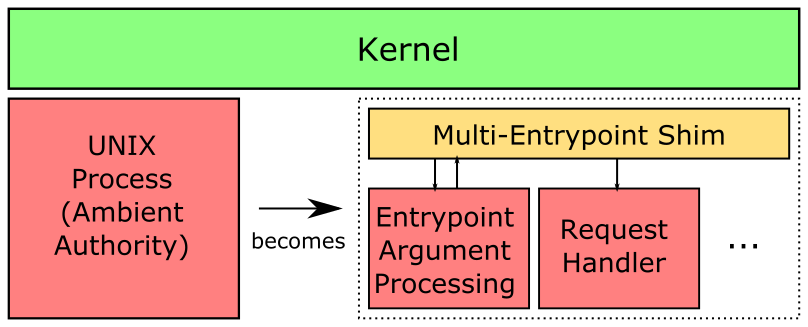
\includegraphics[width=\columnwidth]{figures/self-compartmentalisation-interactions.png}
    \caption{Interaction between the application and the environment.}
    \label{fig:self-compartmentalisation-interactions}
\end{figure}

An example of running a Void Process application is given in Figure \ref{fig:self-compartmentalisation-interactions}. What was originally a monolithic application becomes a set of applications that communicate with a new shim. The shim does not replace the kernel, and instead supplements it with new higher-level abilities. Each entrypoint receives input from the shim, and can return data to the shim where appropriate. Most of this data is in the form of file descriptors, which are treated as capabilities in this system.

A Void Process application stores the requirements for running it as static data in the ELF of the binary. When launched, \texttt{binfmt\_misc} is used to launch the application with the multi-entrypoint shim. The shim decodes this data and sets up processes and inter-process communication (IPC) accordingly.


\section{Building Applications}

\subsection{No Permissions}

The cornerstone of strong process separation is an application that is completely deprivileged. Listing \ref{lst:deprivileged-application} shows an application which, when run under the shim, drops all privileges except \texttt{stdout}. This is easy to achieve under the shim.

\lstset{language=C,caption={An application that requires only stdout and stderr.}}
\begin{lstlisting}[float,label={lst:deprivileged-application}]
#[entrypoint(stdout)]
fn main() { println!("hello world!"); }
\end{lstlisting}

\subsection{gzip}

GNU gzip \citep{gailly_gzip_2020} is well structured for privilege separation, though doesn't implement it by default. There is a clear split between the processing logic, selecting the items to do work on, and the compression/decompression routines, each of which are handed a pair of input and output file descriptors. This is shown by Watson et al. in \cite{watson_capsicum_2010}.

As C does not have high-level language features for multi-entrypoint applications, adapting it is slightly more verbose than the other examples seen. However, the resulting code change is still only X lines, if a bit more intricate. This places the risky compression and decompression routines in full sandboxes, while still allowing the simpler argument processing code ambient authority. The argument processing code needs no additional Linux capabilities to manage this permissioning, as the required capabilities are provided by the shim.

\subsection{TLS Server}

\begin{figure}
    \centering
    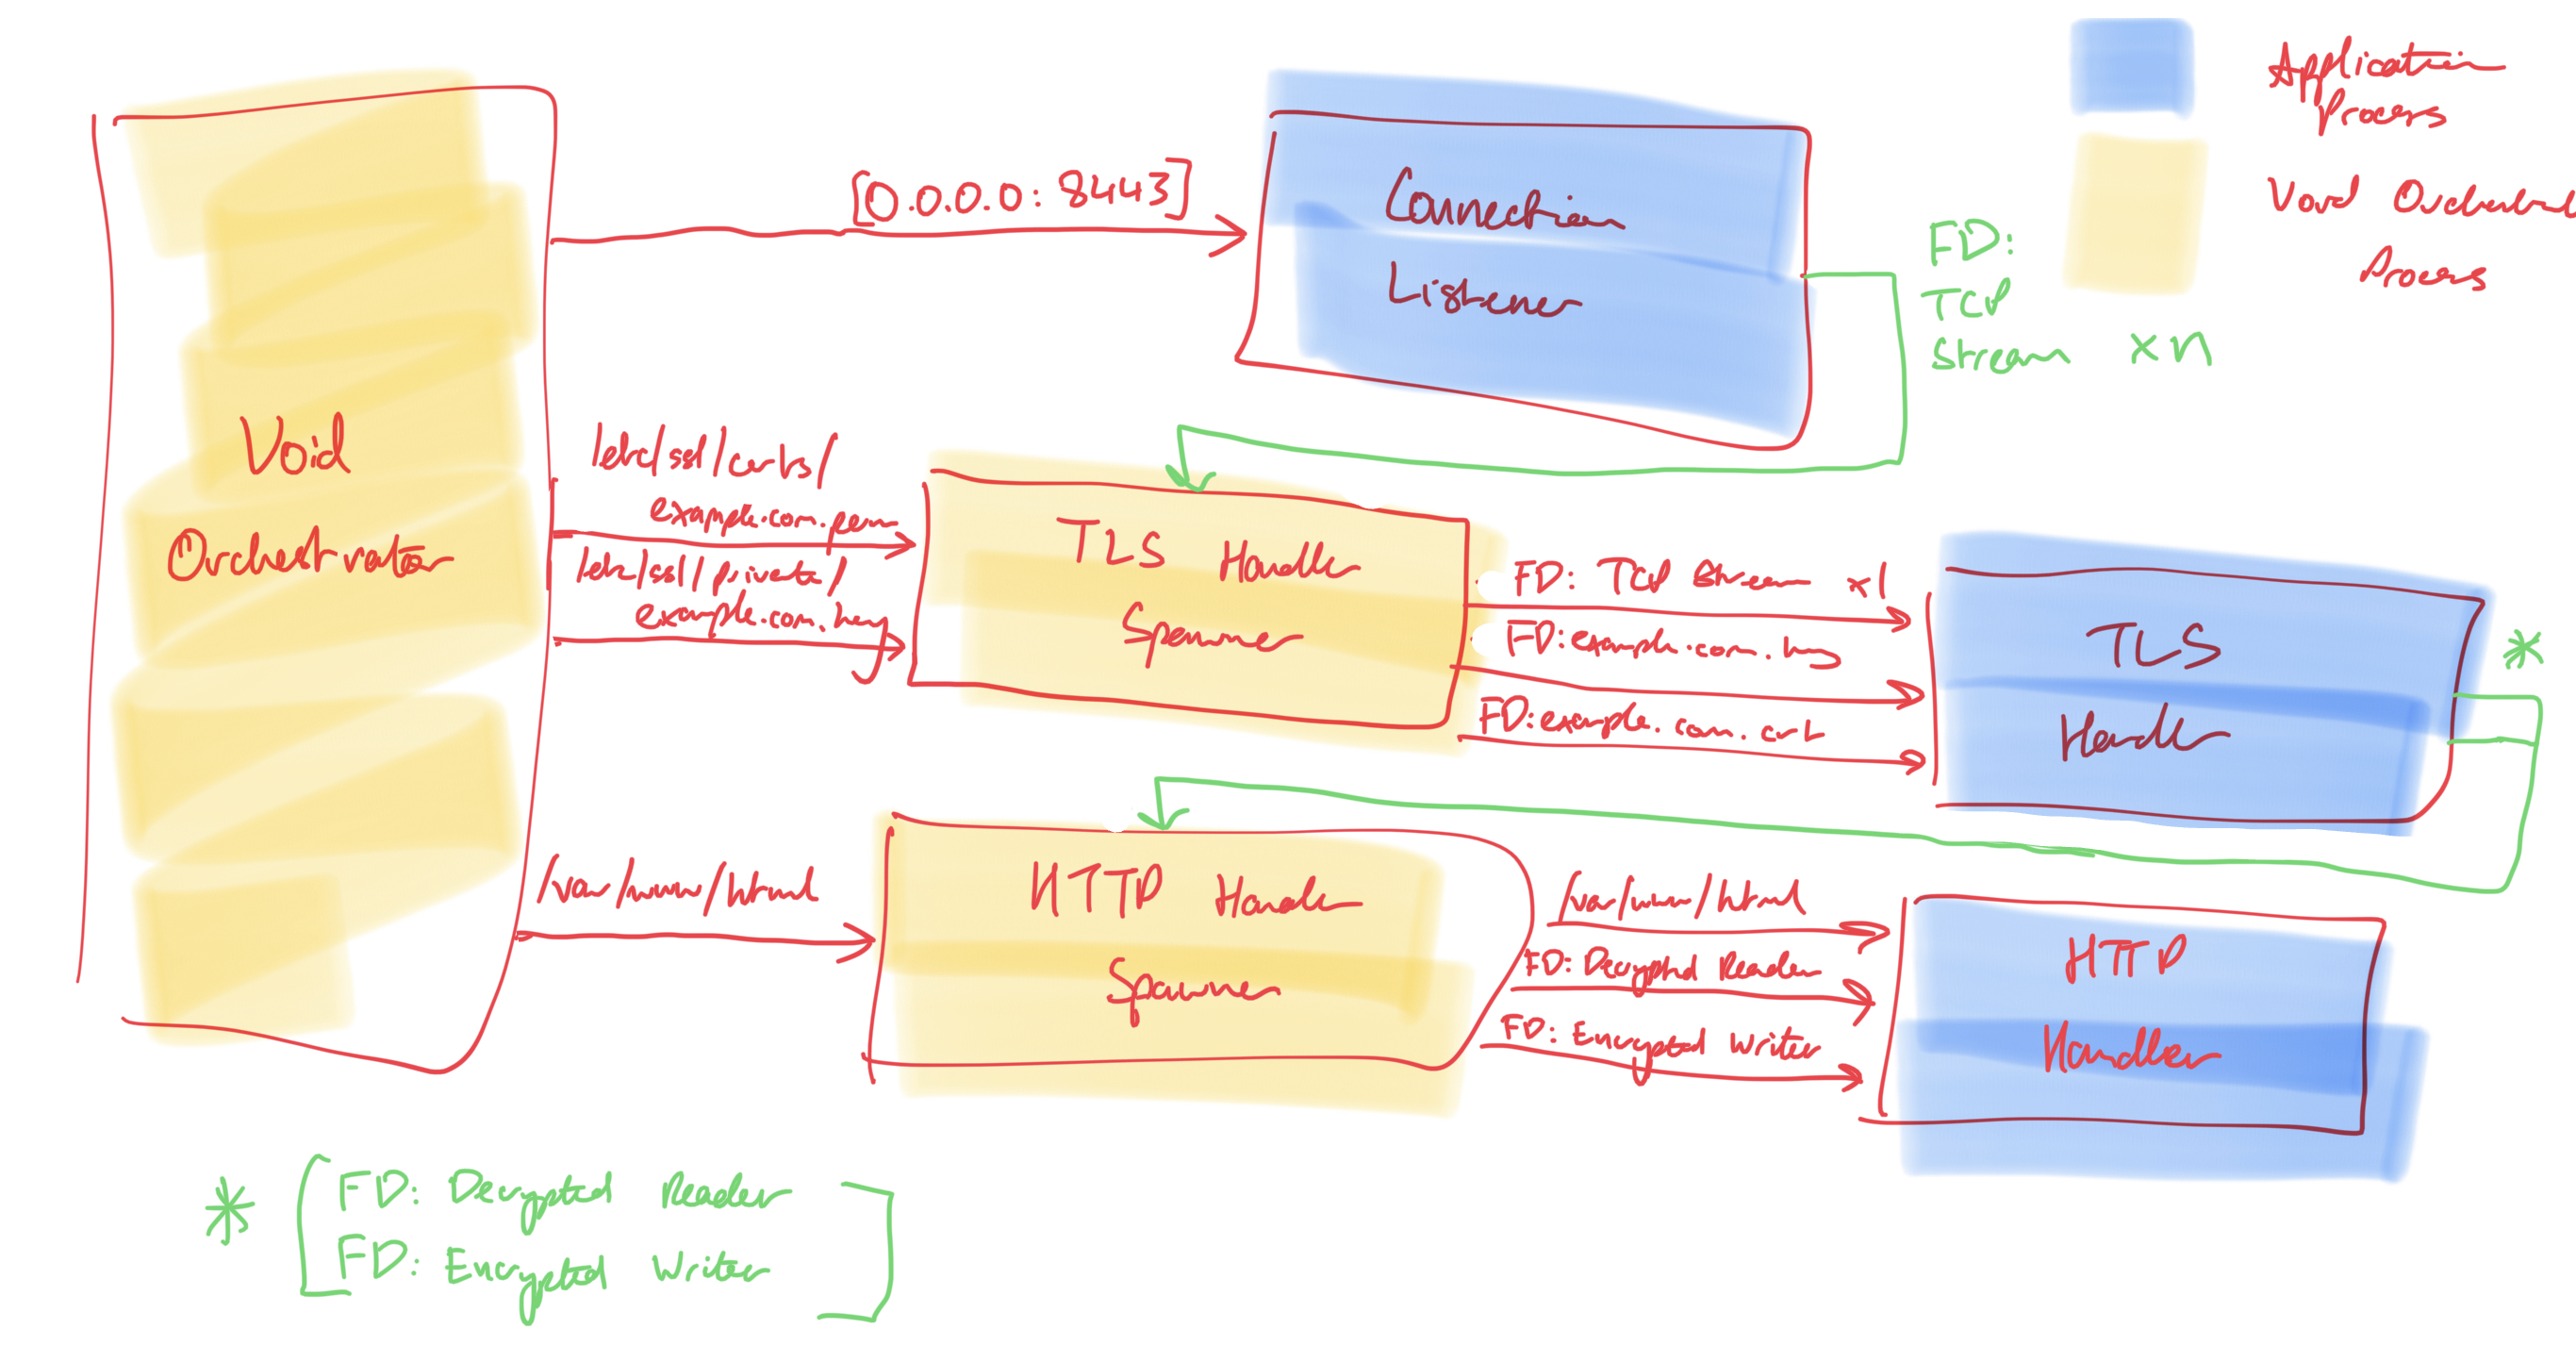
\includegraphics[width=\columnwidth]{figures/tls-server-splitting.png}
    \caption{Process separation in a TLS server.}
    \label{fig:tls-server-splitting}
\end{figure}

Finally, a rudimentary TLS server is created to show the rich privilege separation abilities of multi-entrypoint applications. An example structure is shown in Figure \ref{fig:tls-server-splitting}. Rather than being provided with a view of the network, the initial TCP handling process is given an already bound socket listener by the shim. This allows the TCP handler to live in an extremely restricted zero-access network namespace, while still performing the tasks of receiving new TCP connections.

Next, the TCP handler hands off the new TCP connections to the shim. Though the figure shows this as a direct connection between the TCP handler and the TLS handler, they are passed through the shim, from which the shim spawns a fresh TLS handler for each connection. The TLS handler is handed file descriptors to the certificate and key files that it requires, and hands back a decrypted request reader and an empty response writer file descriptor to the shim.

Finally, this pair of decrypted request reader and response writer are handed to a new process which handles the request. In the example case, this new process is handed a dirfd to \texttt{/var/www/html}, which is bind-mounted into an empty file system namespace by the shim. This allows the request handler enough access to serve files, while restricting access to anything else.


\section{Evaluation}

\todo{Write evaluation}


\section{Related Work}

\subsection{Virtual Machines and Containers}

Virtual Machine solutions \citep{barham_xen_2003,vmware_inc_understanding_2008} provide the ability to split a single machine into multiple virtual machines. When placing a single application in each virtual machine, they are effectively isolated from one another. Full fat container solutions such as Docker \citep{merkel_docker_2014}, containerd [CN], and systemd-nspawn [CN] provide mechanisms to isolate an application almost completely from other applications running on a single machine. Some have claimed that this provides isolation superior to virtual machines \citep{soltesz_container-based_2007}.

Both of these solutions are less effective at isolating parts of an application from itself [CN with research]. Consider running only a TLS web server in a virtual machine. Although other applications will be unable to access the certificates, as they are in different virtual machines, methods within the application that should not be able to access the certificates still can.

While virtual machines and containers provide a strong isolation at the application level, they are not a compelling solution to intra-application privilege separation.

\subsection{systemd}

\texttt{systemd} [CN] provides a declarative interface to all of the process separation techniques used in this work. Rather than the responsibility of the programmer, creating these declarative descriptions is most commonly left to the package maintainers. This work seeks to provide similar capabilities to the people best suited to privilege separating an application: the developers.

\subsection{Capsicum}

Capsicum \citep{watson_capsicum_2010} extends UNIX file descriptors in FreeBSD to reflect the rights on the object they hold. These capabilities may be shared between processes as other file descriptors. The goals of both software are the same: make privilege separated software better. However, we take quite different approaches. Multi-entrypoint applications focus on building a static definition really close to the code, while Capsicum allows processes to dynamically privilege separate. This allows applying static analysis to the policies, while also keeping the definition close to the code.


\section{Future Work}

\subsection{Dynamic Linking}

Dynamic linking works correctly under the shim, however, it currently requires a high level of manual input. Given that the threat model in Section \ref{section:threat-model} specifies trusted binaries, it is feasible to add a pre-spawning phase which appends read-only libraries to the specification for each spawned process automatically before creating appropriate voids. This would allow anything which can link correctly on the host system to link correctly in Void Processes.


\section{Conclusion}

\todo{Write conclusion}

%%
%% The acknowledgments section is defined using the "acks" environment
%% (and NOT an unnumbered section). This ensures the proper
%% identification of the section in the article metadata, and the
%% consistent spelling of the heading.
\begin{acks}
\todo{Write acknowledgements}
\end{acks}

%%
%% The next two lines define the bibliography style to be used, and
%% the bibliography file.
\bibliographystyle{ACM-Reference-Format}
\bibliography{references}

%%
%% If your work has an appendix, this is the place to put it.
\appendix


\end{document}
\endinput
%%
%% End of file `sample-acmsmall.tex'.
